% !TEX root = ../thesis-example.tex
%
\chapter{Related Literature}
\label{sec:related}
Algorithmic trading (hereafter, referred to as AT) has been present since the mid 1990s with the rise of personal computer power and the internet \cite{WEB:PISANI:2010}. Documenting these methods towards the volatile and unregulated market of cryptocurrency (hereafter, referred to as crypto) will address the little related literature present due to the infancy of crypto market. This project hopes to address this gap by applying tested methods used on the stock and currency market, while building a platform to utilise the bot. This chapter will discuss the topics algorithmic trading, trading indicators, crypto and their markets, and relevant development libraries to implement the bot. These topics will provide an understanding of how algorithmic trading is used and why they have become a necessity for the operation of the stock market. Illustrating how these trading methods and trend indicators work will show how they can be used towards AT in crypto. Through my research of the world of crypto, I evaluate why their markets are unique and what can be expected. Lastly, I discuss relevant development libraries that will be useful towards this project. 
% \cleanchapterquote{A picture is worth a thousand words. An interface is worth a thousand pictures.}{Ben Shneiderman}{(Professor for Computer Science)}


\section{Algorithmic Trading}
\label{sec:related:algoTrading}
\noindent Treleaven, Falas and Lalchand \cite{ART:Treleaven:2013} defines AT as "any form of trading using sophisticated algorithms (programmed systems) to automate all or some part of the trade cycle". AT fits into systematic trading, described as trading based on rules. This combines both trend analysis (Sec. \ref{sec:related:algoTrading:tradeprocess}, pg. \pageref{sec:related:algoTrading:tradeprocess}) and high-frequency trading (Sec. \ref{sec:related:algoTrading:HFT},  pg. \pageref{sec:related:algoTrading:HFT}). Nuti, Mirghaemi, Treleaven (who also authored \cite{ART:Treleaven:2013}) and Yingsaeree \cite{ART:Nuti:2011} state AT was designed to automate trade while being profitable and executing orders optimally. These characteristics of AT have allowed it to fit into a wide range of use cases, which is why it is dominant on equity markets, resulting in 90 percent of the total daily trade volume in the EU and US markets today \cite{WEB:Cheng:2017,ART:Kolakowski:2018}. The computational power and accuracy of AT demonstrates as to why this is the case and is seen through my discussions on the process of how trades come to fruition. Illustrating how these steps are taken demonstrate what this project can expect to implement.

\subsection{Trade Process}
\label{sec:related:algoTrading:tradeprocess}
The trade process for AT described by Nuti et al \cite{ART:Nuti:2011} and Treleaven et al  \cite{ART:Treleaven:2013} consists of data access, pre-trade analysis, trading signal generation, trade execution, and post-trade analysis. The listed steps (Fig. \ref{fig:related:tradeprocess}) define key actions required to analyse data to determine if the market conditions can turn a profit in the entry or exit of an asset. The ultimate goal of AT is to gain profit or know when to cut losses, where Nuti et al \cite{ART:Nuti:2011} and Treleaven et al  \cite{ART:Treleaven:2013} agree are addressed by these steps. The research of this trading process capture the fundamental variables required for an algorithm to work, considering all aspects of the market to trade on.

\begin{figure}[htb]
    \centering
	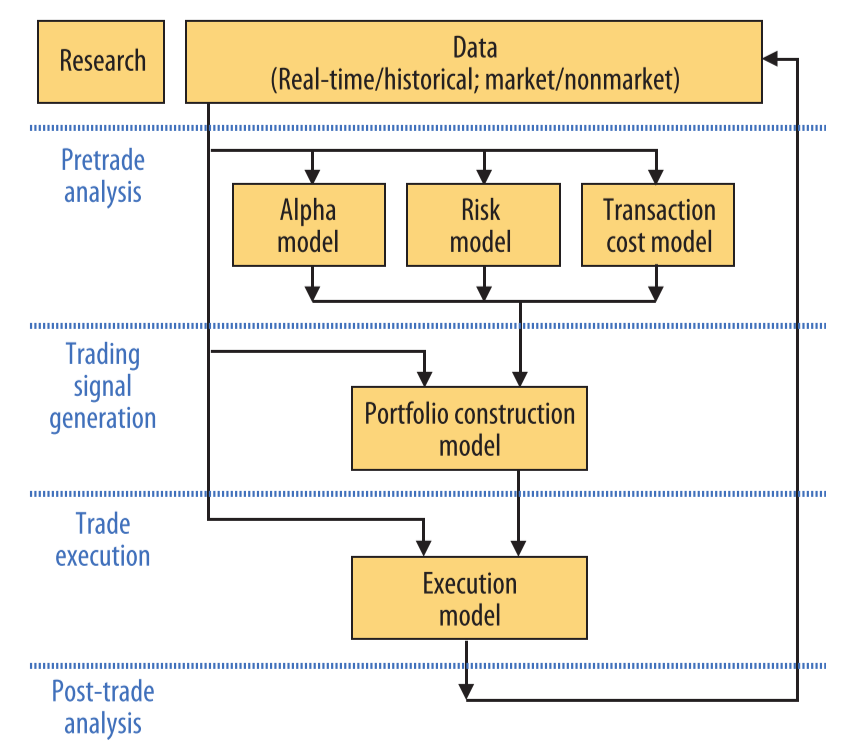
\includegraphics[width=0.55\textwidth]{content/graphics/AT-trade_process}
	\caption{Trade Process Figure by Nuti et al \cite{ART:Nuti:2011}: \textit{(a)} Research / Data, \textit{(b)} Pre-trade Analysis, \textit{(c)} Trading Signal Generation; \textit{(d)} Trade Execution, \textit{(e)} Post-trade Analysis }
	\label{fig:related:tradeprocess}
\end{figure}

Treleaven et al \cite{ART:Treleaven:2013} discuss that access to clean data is crucial to the operation of AT. The specificity of data required depends on the type of algorithm being built. Treleaven et al describe data which can vary from financial, economic, social and news to real-time, historic and analysed market data. The selection and validity of data can greatly affect the operation of AT and requires vetting of cleanliness. This is consistent with Chan's \cite{BOOK:Chan:2013}  discussion of using data to simulate strategies using backtesting, where the results of a strategy may appear positive, but performs poorly when applied to out-sample real-time data. This suggests that the data used in backtesting may be limited, failing to cover the scope of the market. Considering this, implementing a robust system on backtesting that covers various different data sets would ensure the algorithm prevents unforeseen issues.

Both Treleaven et al \cite{ART:Treleaven:2013} and Nuti et al \cite{ART:Nuti:2011} describe that pre-trade analysis discerns trading opportunities from data with the aim of predicting future prices to generate trading signals. Specifics of how this is achieved is discussed in section \ref{sec:related:tradingStrategies} (Pg. \pageref{sec:related:tradingStrategies}), but the three main categories of analysis are fundamental\footnote{Information relating to markets to determine an asset's fair value e.g. interest rates}, technical\footnote{Historic, current, and other market information to predict future prices} and quantitative\footnote{Mathematical models based on treating assets prices as random rather than deterministic (like technical analysis)}. As technical analysis is the aim of this project, the forecast of prices and momentum are based on trend indicators and other market data. Three mathematical models: alpha, risk and transaction cost (Fig. \ref{fig:related:tradeprocess}, part b) are used to predict future behaviour, evaluate levels of risk and determine potential costs induced respectively. Each model is crucial to determine the success rate of the entry into - or exit from - the market, but I would emphasise that the risk model may be the most crucial. Taking precautions to ensure risk is minimised is one of the biggest factors to ensure profitable trades, concluded by Engle, Ferstenberg and Russel \cite{ART:Robert:2012} that majority of traders opt for strategies that are risk averse.

Trading signal generation differs from pretrade analysis, specifically determining the values the trade should execute with. Here is why AT positions 90 percent of the daily trade volume \cite{WEB:Cheng:2017,ART:Kolakowski:2018} with its ability to analyse all market information in milliseconds, allowing it to find the entry points with minimal risk. Nuti et al \cite{ART:Nuti:2011} define two problems that could occur during entry, oscillating buy and sell signals and incorrect model assumptions.  Kaufman \cite{BOOK:Kaufman:2013} discusses indicators (Sec. \ref{sec:related:tradingStrategies}, pg. \pageref{sec:related:tradingStrategies}) that can be unprofitable if oscillating prices are failed to be addressed. High transaction costs and increased losses can occur as a result of this. Detecting when to exit by taking profits or minimising losses is crucial, so by failing to address both of these points could lead to an unprofitable and useless signal. 


Finally, Nuti et al \cite{ART:Nuti:2011} and Treleaven et al \cite{ART:Treleaven:2013} states that trade execution determines the constraints a transaction can occur, such as costs or duration. The main point made at this stage is to not adversely affect the market with large orders, while executing trades with reduced risk. Deciding whether to split large orders up into smaller chunks could prevent a change of market momentum, but prolonging the fulfilment of the order could result in failing to obtain the best price. Considering this, research by Engle et al \cite{ART:Robert:2012} states there is a risk component involved in time taken to execute a transaction. The low liquidity and high volatility of the crypto market would bolsters this risk factor, requiring extra attention to trade executions. 


For example, a market order\footnote{Buying/Selling an asset at the best possible price at the current time} during low liquidity would most likely result in overpaying for an asset and increasing volatility, whereas by placing a limit order\footnote{Buying/Selling an asset for a set price} can allow for a better price to fill over a longer period. However, this can also produce issues such as being cut above by a higher placed limit order, reducing the chances of your order filling at the quoted price. Continued analysis even after a trade has executed is required to minimise risk until the order is filled.

The trading process described by Nuti et al \cite{ART:Nuti:2011} and Treleaven et al \cite{ART:Treleaven:2013} correlates with how an algorithmic trading bot to crypto could be implemented. Using the aforementioned process determines steps at the pre-trade analysis stage to minimise risk while considering how to actually execute the trade. Demonstrating research and discussing common pitfalls of these stages shows how a well-designed trading bot can be implemented using technical analysis. While the trade process is discussed, not much about the actual implementation or success of these systems is mentioned. Taking factors such as risk based on transaction times and costs, and generating trade signals on correct analysis provides steps this project will follow. This paper will also discuss how these steps can be applied to the nascent crypto market, using real data and providing results based on analytics. Although this project looks to build a trading bot based on a form of slower pre-trade analysis, High-Frequency Trading constitutes the bulk of AT used in the stock market today. 

\subsection{High Frequency Trading}
\label{sec:related:algoTrading:HFT}
\noindent  Seth \cite{WEB:SETH:0001} states the largest category of the AT cohort is associated to High-Frequency Trading (hereafter, referred to as HFT). While low-latency HFT is not possible in the crypto market (Sec. \ref{sec:related:cryptoAndTheirMarkets}, pg. \pageref{sec:related:cryptoAndTheirMarkets}) - and not used in the development of this project - discussing the effects that HFT has on the stock market is beneficial to evaluating its health and what the crypto market can expect. HFT is the primary trading type in the modern stock market characterised by the speed and volume of trades it can execute within a small-time frame.

Both Seth \cite{WEB:SETH:0001} and Chorida, Goyal, Lehmann and Saar \cite{REPORT:ChordiaEtAl:2013} state the fundamental requirement for a successful HFT algorithm is low-latency - defined by Chorida et al as "strategies that respond to market events in the millisecond environment". This is evident by trading firms spending substantial amounts to be placed as close as possible to the exchange's server to remove milliseconds off latency times \cite{ART:Aswani:2016}. This allows trading firms to respond to the most recent market data, providing the advantage to the first trader that receives the data. Comparing human ability to analyse and respond in this time-frame displays why HFT is the primary method to transact on the market.

Chorida et al \cite{REPORT:ChordiaEtAl:2013} state that most of the liquidity in the stock market is provided by HFT algorithms based on their identifiable activities. This appears inline with an article by Warmbrodt \cite{ART:Warmbrodt:2016}, however he hinges on this as a defence traders use towards the uncertainty regulators face with volatility from events like the 2010 ``flash crash''. He also explains that Clinton had plans for a financial reform to tax certain types of harmful HFT in her presidential race. This reform would of reduced the profitability of HFT, resulting in less firms using this method which may of potentially hindered market quality. Events like the ``flash crash'' shows the extent of controversy that HFT is facing, with Nuti et al \cite{ART:Nuti:2011} and Treleaven et al \cite{ART:Treleaven:2013} basing this on the lack of knowledge towards how they operate. Warmbrodt \cite{ART:Warmbrodt:2016} discusses the findings from an investigation, calling this `predatory' behaviour from aggressive AT firms. 

However, other officials outline the positives of HFT with Warmbrodt \cite{ART:Warmbrodt:2016} quoting the US `Securities and Exchange Commission' (SEC) Chairwoman stating, "[investors] are doing better in today's algorithmic marketplace than they did in the old manual markets". Warmbrodt adds that this is apparent to lower trade costs present in today's markets. The increased liquidity HFT brings allows for larger orders to be successful close to the current price and execute within a short period.  Bajpai \cite{WEB:Bajpai:0001} builds on this by stating that "liquidity is an important characteristic of a good market". The price difference between the highest buy order and the lowest sell order, also known as the `bid-ask spread', reduces transaction costs by producing smaller differences between the buy and sell prices. This incentivises multiple orders to be made consistently by traders, with little transactional cost. In turn, the market is provided with liquidity which ultimately reduces risk for investors. Whether the effects of HFT on the market is resulted by poor understanding or some exploitative behaviour, further research is required to allow regulators to put protective measures in place. 

While Chorida et al \cite{REPORT:ChordiaEtAl:2013} agrees that when HFT operates correctly it can improve the quality of the market with liquidity, it can also degrade it by demanding liquidity without any market makers to fill this demand. This subsequently increases volatility by occurring a major shift in the assets price. Chorida et al state this is evident by the ``flash crash`` of May 2010 where HFT - while it may not of triggered it - certainly affected price volatility. As most HFT algorithms follow trends, they tend to trade on similar rules. An article by Kolakowski \cite{ART:Kolakowski:2018} describes this as `herd' behaviour on steroids, quoting the director of Exchange-Traded Fund (ETF), "when selling happens, more selling can occur and when buying happens, more buying can occur". This can pull liquidity from the market allowing the price to tumble, especially when AT controls roughly \$8.8 trillion according to a 2016 study \cite{ART:Kolakowski:2018}. 

A source from Anagnostidis \cite{UNPUB:Anagnostidis:2017} explains "the speed with which the quotes are posted and cancelled has been criticised by market participants because its creates a false sense of deep liquidity supply for a stock". While this seems to counter previous points of HFT supplying liquidity, it's important to emphasise this is referring to \textit{deep} liquidity. It is undeniable that HFT provides vast amounts of liquidity as mentioned above. Anagnostidis summarises by stating that liquidity generated by submissions and cancellations does not translate into a persistent effect on liquidity supply. This false cushion of liquidity is derived by the current rules followed HFT algorithms and their herd like behaviour as discussed by Kolakowski \cite{ART:Kolakowski:2018}. This can greatly impact the stability of the market as a whole and is the main source for concern about HFT's affect to regulators \cite{WEB:Kaufman:2016}.   

However, this method of `submit-cancel` is also used for price discovery\footnote{Determining price of asset based on analysis of buyer and sellers} of an asset due to AT's precise market analysis. It provides informative predictions based on all market information available leading to readjustment of order prices. An empirical study by Brogaard, Hendershott and Riordan \cite{UNPUB:Brogaard:2017} concluded that HFT improves pricing efficiency\footnote{The assets price is best reflected by all information possessed} by "trading in the price's permanent direction and against transitory pricing errors". This is inline with another empirical study by Benos and Sagade \cite{ART:BENOS:2016} stating non-passive HFT flows in the direction of future price changes. It becomes apparent that price discovery and efficiency is improved by HFT as they tend to follow market trends.  

HFT is possible in the crypto markets but not to the same extent as the equity market. The lack of low-latency connections partially prevents the evident positive and negative effects described above. While tightening spreads, reducing transaction costs, improving price discovery and strengthening price efficiency would contribute to the market's health overall, it is still in an unknown area of regulation to prevent negative damage. This leaves low-latency HFT producing damaging effects with the described `herd' mentality contributing to the rise of flash crashes.  However, with the crypto market still being unregulated with extreme volatility, perhaps employing low-latency HFT could still improve upon the current market's quality. Ultimately, the adverse effects are resulted by the domination of AT in the equity market over many years of development. Perhaps by the time crypto establishes and grows it's market, better regulation for itself and HFT could be further developed.



\section{Trading Strategies}
\label{sec:related:tradingStrategies}
\noindent As discussed in the trade process (Sec. \ref{sec:related:algoTrading:tradeprocess}, pg. \pageref{sec:related:algoTrading:tradeprocess}), a well defined trading strategy is the basis of pre-trade analysis. Lien \cite{BOOK:Lien:2016} states that technical analysis works well in the fiat currency\footnote{Legal tender which does not have intrinsic value but declared to have value by the government} market due to its speculative nature and its tendency to overshoot and correct.  Most literature on technical analysis is based on developed equity and currency markets with the discussion on the crypto market being sparse. These handful of related works apply similar indicators that Lien discusses with success, so by evaluating work intended for developed markets will show what trends can be used in the crypto market. This will provide market interpretation for this project and the construction of a sound strategy. I discuss similarities between crypto and other markets in section \ref{sec:related:cryptoAndTheirMarkets} (Pg. \pageref{sec:related:cryptoAndTheirMarkets}).

A paper from Tapa, Yean and Ahmed \cite{ART:Tapa:2016} concluded through their use of moving averages that they were able to return profit on a simple crossover moving average strategy. This single use shows promising results towards the scope of this project, suggesting that technical analysis can be applied effectively to real-time market data. The moving average indicator is one of the most popular identifiers to market momentum by providing clear trends. Kaufman \cite{BOOK:Kaufman:2013}, Lien \cite{BOOK:Lien:2016} and Harmon \cite{BOOK:Harmon:2014} discuss how to apply moving averages and other indicators in practical ways to achieve profitable results. I will also look at the relative strength index (RSI) and moving average convergence/divergence (MACD) momentum indicators and Bollinger Bands (BB) to discuss their beneficial uses toward analysis of market trends.

A moving average (MA) is the mean of closing prices on intervals over a defined period - e.g. 12 days - and is described by Kaufman \cite{BOOK:Kaufman:2013} to remove market noise and find the direction of the price. The most common MA is the simple MA (SMA) which produces an average deduced by all the previous prices with equal weighting. Kaufman \cite{BOOK:Kaufman:2013} states that the SMA can have abrupt changes in value when a significant price movement is dropped off the end due to this equal weighting. This may cause false signals to be generated if recent prices exhibit little change and the older data point had great significance. This could be exceptionally import towards the crypto market due to the extreme volatility they can produce, such as a 15 percent increase in price within a few minutes. 

However, more responsive MAs may suit the crypto market such as the exponential moving average (EMA) suggested by Kaufman \cite{BOOK:Kaufman:2013}, being summarised to give greater weighting to more recent prices. Thus, the effect of dropping off the end price is reduced. This would suggest an improved effectiveness compared to SMA at predicting an accurate trend in the current market price. Harmon \cite{BOOK:Harmon:2014} suggests that using a smaller time-frame with SMA than using an EMA could provide similar results, although, he presents no justification or acknowledgement to the SMA drop-off issue and seems to be merited on opinion. This contrasts with Kaufman's \cite{BOOK:Kaufman:2013} suggestion of using an EMA, however, addresses and expands on this issue with justification. It is worth noting that EMAs are used frequently in other indicators, as I discuss later in this section.
%BOOK Technical Analysis: The Complete Resource for Financial Market Technicians uses Kaufy as a reffy
    
While the SMA can be responsive to the current market price, the weighting of previous prices being equivalent to the current price results in a smooth trend line indicator. Whereas, EMA responds quicker to the current market price, but due to lower weighting of older prices results in a more jagged trend line. I lean more towards EMA to give the best insight towards market trends due to the volatility of crypto's market conditions and hence the need to react to these price changes quickly. However, the use, analysis, and comparison of both MAs in this project will be beneficial to draw conclusions as to which is more effective towards crypto.

Nonetheless, the MA is proven through multiple research papers including Wong, Manzur, and Chew \cite{ART:Wong:2003} who concluded single, dual, and triple MAs produced positive results on the Singapore stock market. They acknowledge that a sideways moving market or times of excessive volatility would generate false signals. Applying the MA by itself to the crypto market may not produce similar results due to its volatile characteristic, so the conjunction of multiple indicators will be required to confirm trends.  

Kaufman \cite{BOOK:Kaufman:2013} describes that the RSI indicates when overbought or oversold conditions occur. This is determined by dividing the total upward price changes over the total downward price changes from a period of time, and then fitted into a range of 0 to 100. This gives the measurement of the current price movement's relative strength over the defined period. This indicator will help determine if a trend reversal is likely to happen based on exceeding or dipping below the threshold values 70 and 30 respectively. Lien \cite{BOOK:Lien:2016} illustrates an example of using RSI to identify when to enter the market. 

\begin{figure}[htb]
    \centering
	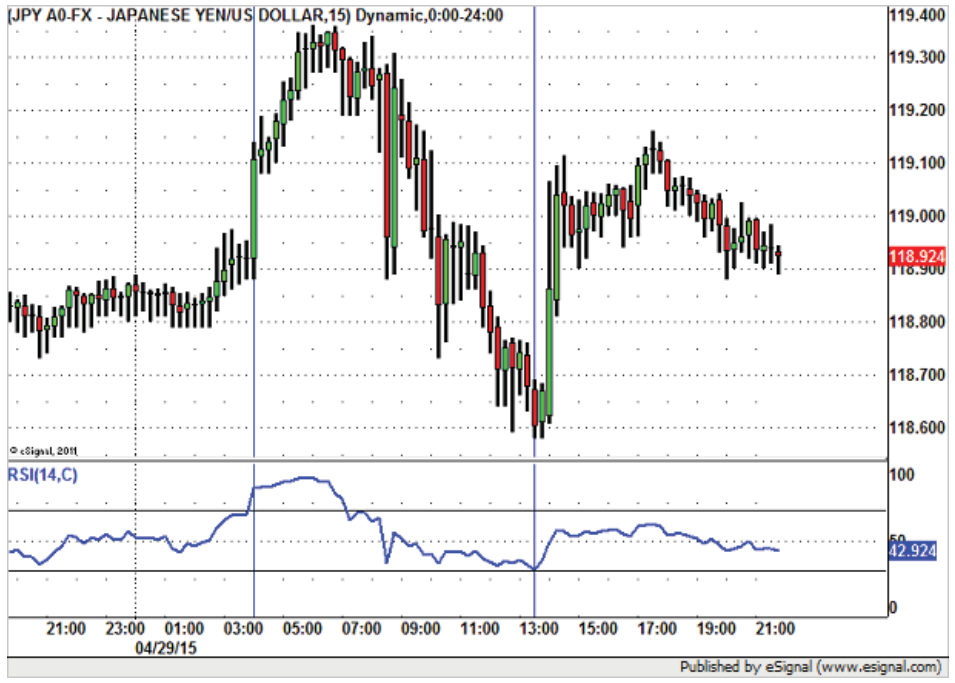
\includegraphics[width=0.7\textwidth]{content/graphics/USDJPY-15_min_chart}
	\caption{USDJPY 15 minute chart by Lien \cite{BOOK:Lien:2016}: \textit{(a)} RSI above 70 at 03:00
	\textit{(b)} RSI at 30 at 13:00}
	\label{fig:related:USDJPY_15min}
\end{figure}

Entering the market at figure \ref{fig:related:USDJPY_15min}.a when the RSI value was above 70 would of seen a market reversal against the entry trade. Waiting until figure \ref{fig:related:USDJPY_15min}.b was the better entry time with the RSI at 30. Although, Kaufman \cite{BOOK:Kaufman:2013} also states that in a study the average amount of RSI values ranges from the 32 to 72 market. He continues, showing that roughly 50 percent of RSI values fall between this range, indicating that the thresholds may need to be widened. Suggestions of 80 to 20 or 85 to 15 are considered extremely strong indicators as they are hard values to sustain. While the example for figure \ref{fig:related:USDJPY_15min} was an ideal scenario, it would be naive to assume this is always the case. Experimenting with threshold ranges to fit this indicator towards the crypto market will be a research point this project looks into.

The MACD is the difference of two EMAs - usually based on 12 (short) and 26 day (long) periods - and another EMA - usually 9 days - that generate trade signals when the lines intersect. Both Harmon \cite{BOOK:Harmon:2014} and Kaufman \cite{BOOK:Kaufman:2013} evaluate the effectiveness of this indicator to be unreliable for trading as it would require the constant fitting of threshold lines to prevent whipsaws\footnote{A volatile price action in which a security swings back and forth in a chaotic pattern}. It would seem that this strategy would work well in an upward or downward market interval, but it would result in poor trades in a sideways market due to whipsaws of the trend line intersections. They state that MACDs are ultimately used to define divergence signals.

Utilising both RSI and MACD in this project's trading strategy will indicate if market reversals are likely to occur or if momentum is still heading in a certain direction. A point Lien \cite{BOOK:Lien:2016} emphasises is the importance of utilising multiple time frames with these indicators as to understand the bigger picture of the market. Failing to analyse where the current moment in the market is can lead to poor trades on the larger scale. Both Kaufman \cite{BOOK:Kaufman:2013} and Harmon \cite{BOOK:Harmon:2014} also discuss this point and conclude that analysis of multiple time frames is important to clarify the current direction of the market.

Another trend indicator which defines oversold or overbought market conditions is the Bollinger Band (BB). It is constructed with three MAs usually based on a 20-day SMA with similar upper and lower bands. The bands are created by adding or deducting the double of the standard deviation of the price over a 20-day period.  Harmon \cite{BOOK:Harmon:2014} analyses the BB to indicate extreme or slight volatility in the price of stocks, discussing when the BB `squeezes' - the upper and lower bands narrow - that volatility has moved out of the stock, indicating a significant price movement is about to occur. 

Harmon \cite{BOOK:Harmon:2014} explains that the price breaking through the upper or lower band indicates an overbought or oversold signal. He states it can be then be used for a trade a signal when the price closes under/above the upper/lower band, confirming a reversal in the trend. This is similar to a strategy Kaufman \cite{BOOK:Kaufman:2013} describes, however he states that the characteristic of a price closing above the upper band ensues a continued trend in an upward trajectory for a few days. This is not conveyed by Harmon \cite{BOOK:Harmon:2014} as he explains the reversal follows shortly after the break through. 

An example of Kaufman's strategy seen in figure \ref{fig:related:BB_trade_strat} would illicit a buy signal when the price closes above the upper band and longing for a period, then shorting when the price closes below the lower band. If the price closes below the middle MA while still longing, the position is closed out as a price reversal is likely, which fits to Harmon's \cite{BOOK:Harmon:2014} strategy but is used to minimise risk rather than a trading rule.

\begin{figure}[htb]
    \centering
	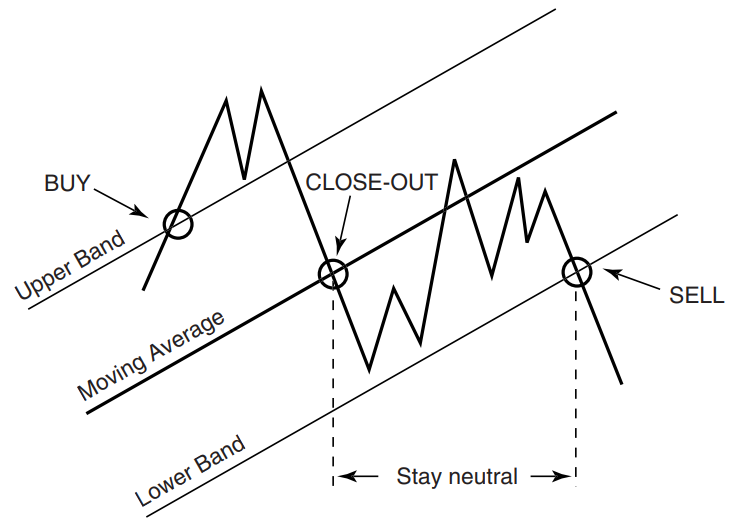
\includegraphics[width=0.6\textwidth]{content/graphics/BB_Trade_Strat}
	\caption{Bollinger Band Trade Signals by Kaufman \cite{BOOK:Kaufman:2013}: 
	\textit{(a)} Buy when price closes above Upper Band
	\textit{(b)} Close position when still longing and price closes below MA
    \textit{(c)} Sell when price closes above Lower Band when shorting}
	\label{fig:related:BB_trade_strat}
\end{figure}

Conversely, the described method by Harmon \cite{BOOK:Harmon:2014} and Kaufman \cite{BOOK:Kaufman:2013} is discouraged by Lien \cite{BOOK:Lien:2016} who explains it's too risky and that two BBs would produce a better strategy. This is the addition of another upper and lower SMA using only the standard deviation of the price. The general rule of thumb is to buy when a trade closes above the first upper band and sell when it trades below the first lower band. Lien describes that while this may not pick the `perfect' bottom, it can avoid a premature entry into an asset. The heightened precautions of the double BB would ultimately minimise risk when using BBs for trade signal generation. Kaufman \cite{BOOK:Kaufman:2013} notes the high risk involved with the trading strategy based on the single BB, strengthening Lien's criticism of this strategy.

Furthermore, Lien \cite{BOOK:Lien:2016} discusses the use of the double BB to indicate when a currency is trending or ranging\footnote{When a price is osculating between similar prices and heading in no clear direction}. This allows to clearly identify the current movements of the market, aiding in the generation of a trading signal. Ultimately, the point of minimised risk deduced from Lien would indicate towards a safer trading strategy while providing clear interpretations of the market. 

The discussion by Kaufman \cite{BOOK:Kaufman:2013}, Harmon \cite{BOOK:Harmon:2014} and Lien \cite{BOOK:Lien:2016} identify trading strategies through the trend indicators described above. Most of the indicators are based on variations of the MA which interprets clear trends the market is currently in. The described indicators, while only capturing the basics of technical analysis, will satisfy the scope of this dissertation by providing clear trade signal generation. While certain strategies can be executed with one indicator, a common point emphasised is the use of a variety of different indicators. Multiple indicators confirming the same trends would provide a stronger signal generation than an individual signal. 


\section{Cryptocurrencies And Their Markets}
\label{sec:related:cryptoAndTheirMarkets}
% Talk about crypto responding to news and biased trading
% Crpyto is in between currency and securities like stocks, discuss this

\noindent The first cryptocurrency, Bitcoin, made its debut in 2009 with the release of its code base and white paper. This sparked the cryptocurrency market into life which peaked at roughly \$800 billion during its peak in early 2018. It has been reported that the crypto bubble has burst with the current market cap now shy of \$200 billion at the time of writing. Others claim this is just the beginning of a digital currency revolution with the market cap vastly distant from the dot-com bubble where internet stocks were valued at several trillion dollars \cite{ART:Kharpal:2018}. The unpredictability towards crypto's future is attributed by it's uncertainty towards regulation and where it fits into the existing markets. By evaluating this unique market, I can determine if it is profitable, what levels of risk are present and what crypto characteristics to avoid.

From the start of 2017, Bitcoin was worth around \$720. By December it had increased 1,332\% to a peak worth of \$19,783.21 \cite{ART:ELLIS:2018}. This level of movement is unheard of in the equity or currency market, emphasising the extreme volatility of crypto. Last years bull run can be construed as a sudden rush of excitement for the market, which died off after, what Ellis and Swanson \cite{ART:ELLIS:2018} describe as, the price plummeting 66\% (\$6,436). In recent months multiple attempts of reviving the market has taken place by enticing regulation such as multiple Bitcoin ETF proposals to introduce it onto the equity market. The SEC rejected 9 of these proposals which Swanson \cite{ART:ELLIS:2018} claims is due to the concern of lack of transparency and protection for investors. He also mentions that the SEC has concerns of bots manipulating the prices and that exchanges are vulnerable to this manipulation. These are valid concerns as to why Bitcoin is not ready for the equity market, with no protection against volatile price swings and high levels of risk for investors. This ultimately prevents institutional money entering the market and providing stability. 

Vigna and Osipovich \cite{ART:VIGNA:2018} build on this argument stating that some bots are using manipulative `spoofing' strategies. This was outlawed in the US in 2010 but is currently being used to abuse the crypto market. They base this argument around exchanges failing to implement counter measures towards these price jumps, stating "when any venue tolerates manipulative or abusive conduct, the integrity of the entire market is at risk." This ties in with Ellis and Swanson's article \cite{ART:ELLIS:2018} on the SEC's concern towards protection against this market if exchanges are allowing this abuse. 

Other abusive behaviour towards the market can be seen in similar `pump and dump' schemes which Vigna and Osipovich \cite{ART:VIGNA:2018} state generated `\$825 million' over a six month period. This is when a large group of users target a coin, buy a vast portion of the order book and send the price shooting upwards. Then shortly after, they sell at the new high causing the price to plummet while gaining a huge profit. While the market remains unregulated, abusive bots and schemes will exploit it using illegal activities. The effects of these behaviours leaves other traders at a high level of risk, and effects the markets health as a whole.

This is vastly different from regulated markets which monitor for illegal activities \cite{ART:VIGNA:2018}, protecting traders from drastic turns in the market. This attracts large trading institutions to a market with low risk and is why they are avoiding the crypto market. A report by RBC venture capital predicts the crypto market could be worth `\$15 trillion' within 15 years, however it has to first over come risks towards investors. This is why some exchanges are heading down a self-regulatory path, as discussed by Wolfson \cite{ART:WOLFSON:2018}, referring to the Bakkt\footnote{https://www.bakkt.com/} exchange which is in development by Intercontinental Exchange\footnote{https://www.intercontinentalexchange.com/}. This company spawned the New York Stock Exchange (NYSE) and has the infrastructure and experience to bring institutional money with its release. This will bring crypto closer towards regulation, filtering abusive strategies from the market and providing stability.

However, while these developments bring promise they are still a ways off from helping today's market. Swanson \cite{ART:ELLIS:2018} states that big countries are still trying to understand how to properly classify crypto, whether it is a commodity, currency or security. This is due to the multitude of use cases these coins are used for. Some coins are tied to physical assets like oil (Venezeula's Petro Crypto) which, Wolfson \cite{ART:WOLFSON:2018} states bring adherent value and hence liquidity and stability. Other coins are backed one-to-one to a fiat currency (USDT Crypto), and are noted as stable coins due to having this tied value. Some coins are used as utility tokens (IOTA Crypto), to be spent in transactions such as communicating with the Internet of Things (IOT). This conclusively means that different types of coins are valued by different fundamentals and so cannot fit into one specific classification or can necessarily be traded in the same way. An article by Pisani \cite{ART:PISANI:2018} reports a source from the SEC states that Bitcoin is not a security because of its key characteristic of decentralisation. As there is no party that can control it, there is no protection of the asset.

All the aforementioned points will require detailed levels of risk evaluation while stepping through the trade process (Sec. \ref{sec:related:algoTrading:tradeprocess}, pg. \pageref{sec:related:algoTrading:tradeprocess}). Understanding why volatility is so apparent in this market can prepare for the development of this project by being wary of these abusive techniques. Although, as these abusive techniques may look negative towards a regulatory stand point, they don't reflect the profitability that the crypto market holds. Research cited in section \ref{sec:related:tradingStrategies} (Pg. \ref{sec:related:tradingStrategies}) shows that technical analysis can be applied to the crypto market effectively. Pump and dump schemes discussed by Vigna and Osipovich \cite{ART:VIGNA:2018} mostly target low-cap coins as their prices can be moved with relative ease. They rarely target high-cap coins like Bitcoin as they would require a lot of money to move it. A simple resolution to avoid encountering this type of abusive behaviour is to select specific coins that have a high level of liquidity, high trading volumes, and high market caps. As the time of writing, Bitcoin, Ripple and Ethereum are the top three market caps at \$92, \$19, and \$16 billion\footnote{Taken from https://coinmarketcap.com/}.  


As discussed in section \ref{sec:related:algoTrading:HFT} (Pg. \ref{sec:related:algoTrading:HFT}), Chorida et al \cite{REPORT:ChordiaEtAl:2013} state low-latency millisecond transactions are essential to the stock market. However, this is not the case for the crypto market due to the inadequate latency times and heavy network restrictions set by crypto exchanges. Bloomberg's Levine reports \cite{WEB:Levine:2018} that only recently updates coming from the largest US based crypto exchange - Coinbase\footnote{https://www.coinbase.com/} - are betting on becoming the first to support low-latency HFT by offering colocation\footnote{Locating computers owned by trading firms inside the same area as the exchange's servers}. This scarcity of low-latency communication between exchange and trader pushes institutional investment further from the market as they can't utilise their trading methods fully.

An article by Meyer and Rennison \cite{ART:Meyer:2017} state that large proprietary HFT firms DRW, Jump Trading, DV Trading and Hehmeyer Trading have entered the crypto market. It would be clear to assume that DRW and others have only entered this space if there is profit to be made. This is due to some HFT strategies not requiring transactions to occur on the millisecond time frame. This suggests that low-latency is not a fundamental requirement for HFT to be successful in the crypto market and the use of other strategies can also be utilised. Literature on algorithms applying technical analysis to the crypto market are sparse, however technical analysis can be applied towards the market successfully as discussed in section \ref{sec:related:tradingStrategies} (Pg. \pageref{sec:related:tradingStrategies}).


It is a common theme from these articles that a full institutional entrance into the crypto market is still a long way off and that regulators are unsure of how to tackle it. With the lack of regulation, avoidance from most institutions and poor infrastructure ultimately marks the crypto market as being a volatile and manipulated entity. However, this does not mean that the crypto market is unprofitable, which Dyhrberg, Foley and Svec \cite{ART:Dyhrberg:2018} conclude in a study that, specifically Bitcoin, has low trading costs and narrower spreads than major equity markets and declare that Bitcoin is investible. Tying this with other aforementioned points, eludes to the careful selection of the coin to be traded on is critical. With this, it is conclusive to avoid low market cap, low volume and illiquid coins. 

\section{Development Libraries}
\label{sec:related:developmentLibraries}

Python is the development language for this project due to its simple syntax and vast number of powerful libraries. The project looks to analyse large quantities of data and make decisions based on this analysis quickly. This requires the use of a fast data structures and analysis which can be fulfilled by the \textit{pandas} \cite{WEB:PANDAS} library. The back testing of the implemented strategies is also a fundamental step of testing as discussed in section \ref{sec:related:tradingStrategies} (Pg. \pageref{sec:related:tradingStrategies}). The library \textit{Backtrader} \cite{MISC:BACKTRADER} can fulfil this requirement. As this project ultimately looks to build a trading bot web application, basic server side implementation is a requirement. Thus, \textit{flask}\footnote{http://flask.pocoo.org/}  will be used to implement a basic API to interact with the bot. Finally, the data used in the project will be provided by the Binance API \cite{WEB:BINANCE_API:2018}. The \textit{Python-Binance} wrapper by McHardy \cite{MISC:Python-Binance} will be used to handle the communications between the bot and their servers as the wrapper has been approved by Binance.

The \textit{pandas} library is listed to deliver "high-performance, easy-to-use data structures and data analysis tools" \cite{WEB:PANDAS}. It consists of two main data structures, Series and DataFrame, with easy selection, merging, computation and date/time series functionality. This library is described by Li \cite{ART:LI:2018} to be "one of the most popular tools for trading strategy development". He explains how stock data can be imported into the DataFrame structure and automatically parsed to be mutable (App. \ref{sec:appendix:code_snippets}, code snippet \ref{code:rel:dev_lib:pandas:amz_data}). One line of code can read external data, parse it and place it into \textit{pandas'} highly changeable and powerful structure. Their documentation is concise, up-to-date, and rich in detail.

The \textit{Backtrader} \cite{MISC:BACKTRADER} library is ultimately used to back-test trading strategies (Sec. \ref{sec:related:tradingStrategies}, pg. \pageref{sec:related:tradingStrategies}) on historical data. The library summarises itself to save time on building code infrastructure and start building trading strategies off of their customisable indicators. They advertise a vast range of coding features to ensure development is simple, such as familiar constructs to get the difference between two MAs (App. \ref{sec:appendix:code_snippets}, code snippet \ref{code:rel:dev_lib:backtrader:sma_diff}). There is support for multiple other built-in indicators such as the BB, RSI, MACD and EMA that is discussed in section \ref{sec:related:tradingStrategies} (Pg. \pageref{sec:related:tradingStrategies}). There is also integrated support with \textit{pandas}. This allows for the combination of both libraries to work seamlessly with each other, avoiding incompatibility issues. This library addresses Chan's \cite{BOOK:Chan:2013} (Sec. \ref{sec:related:algoTrading:tradeprocess}, pg. \pageref{sec:related:algoTrading:tradeprocess}) point on backtesting to ensure a strategy will work with a wide range of in-sample data.

\textit{Flask} is a micro-framework for Python in the use of web development \cite{MISC:FLASK}. As the ultimate goal of this project is to develop a web application for this trading bot, basic web development structures should be considered. However, for the scope of the dissertation, \textit{Flask} will be mostly utilised for a RESTful API integration to the bot and provide modularity so the project can ultimately be tied in with a front-end. 

There is an extension \textit{Flask} offers named \textit{Flask-RESTful} that provides a lightweight implementation of a RESTful API setup. There documentation demonstrates the minimal code required to prepare specific routes to interact with the server (App. \ref{sec:appendix:code_snippets}, code snippet \ref{code:rel:dev_lib:flask:flask_restful}). As \textit{Flask} is a framework, there is support for multiple other extensions. Thus, developing the web server integration should be minimal, straightforward, and integrate without complication. As McHardy \cite{MISC:Python-Binance} implements a python-wrapper to communicate with the Binance exchange's API \cite{WEB:BINANCE_API:2018}, the streaming of specific coin pairs (e.g. BTC / USDT\footnote{This represents Bitcoin traded against USDT}) market data, their intervals, and a multitude of other options are easily configurable.  


\section{Conclusion}
\label{sec:related:conclusion}


\noindent Set out by the project's aims, research on relevant literature review of AT (Pg. \pageref{sec:related:algoTrading}), the equity, currency and crypto (Pg. \pageref{sec:related:cryptoAndTheirMarkets}) market, technical indicators that identify market trends (Pg. \pageref{sec:related:tradingStrategies}), and the relevant development libraries (Pg. \pageref{sec:related:developmentLibraries}) have been presented. 

Based on this research, a web app can be developed while considering the difficulties that the crypto market produces. Discussing Treleaven et al \cite{ART:Treleaven:2013} and Nuti et al's \cite{ART:Nuti:2011} in depth analysis of the trade process (Sec. \ref{sec:related:algoTrading:tradeprocess}, pg. \pageref{sec:related:algoTrading:tradeprocess}) prepares the core fundamentals required to implement an AT bot. Establishing the point of using reliable, coherent data ensures that the bot can base decisions on trusted sources. This ties together with Chan's \cite{BOOK:Chan:2013} discussion that whole data is required to apply strategies effectively to the real-time market. This is reflected in our preparation of libraries for this project, where \textit{Backtrader} (Pg. \ref{sec:related:developmentLibraries}) provides a resolution to this concern. 

Furthermore, the evaluation of trend indicators prepares this project with the knowledge of how to analyse the market. This is crucial to developing the basics of an AT bot, which can be fitted towards the crypto market by the evaluation of the crypto market itself. Understanding it's current place in the regulatory area provides clarity to what market this project is dealing with. Discussing  low-latency HFT and its scarcity in the crypto market justifies the development of a TA trading bot, while showing comprehension towards - and awareness to - the future of the crypto market.

Future areas of study should analyse the difference of applying TA between equity markets and the crypto market. This can outline the main differences between the markets to inform future researchers who are approaching developments of similar projects. With more work being applied to the crypto market, the development of its the legal standpoint can be addressed as awareness of this upcoming area grows.




